\subsection{Physics model}
\label{sec:physics_model}

\subsubsection{General requirements}

\begin{quote}
``Equations need to be applicable to arbitrary aspect ratio devices.''
\end{quote}

The equations employed will not generically make the assumption of small
inverse aspect ratio.

\begin{quote}
The collision operators between plasma components, plasma and
impurities and plasma and neutrals have to be sufficiently accurate to properly
describe the radiation generated and the energy transfer between species.
\end{quote}

These operators may be included in the model being
derived in FM-WP2, but at this stage simpler model operators are being used.

\begin{quote}
``Photon opacity effects need to be included in the model.''
\end{quote}

The treatment of effects due to radiation are discussed in Annex~A of~\cite{pappeqs2}
(``the equations document"). Initial implementation will account only for
usage~(1) \emph{the calculation of source/loss terms}, with usage~(2) \emph{the production
of synthetic spectra}, depending very much on input from experimentalists,
as anticipated in the science plan~\cite[p\.\,11]{sciplan}.

\begin{quote}
``The equations need to be capable of dealing with multiple species in
non-trace amounts (at least D, T, He and seeding impurities).''
\end{quote}

The models being derived support distribution functions for multiple species.

\begin{quote}
``The equations should not rely on the Boussinesq approximation.''
\end{quote}

The model derived in FM-WP2 does not use the Boussinesq approximation.
Technically, this means \nep\ will need to be able to invert three-dimensional
elliptic operators with non-constant coefficients.
This capability will be available.

\begin{quote}
``The code should evolve both the electron and ion energy (temperature).''
\end{quote}
This is the case with the FM-WP2 model.

\begin{quote}
``It would be acceptable to have only axisymmetric equilibria,
potentially corrected through small perturbations.''
\end{quote}
This is answered by the discussion in \Sec{geometry}.


\subsubsection{High fidelity simulations}
\begin{quote}
``In high fidelity simulations, the kinetic/fluid transition for both plasma and
neutrals has to be properly captured, potentially using a multi-region approach
exploiting different models in different parts of the machine could be
considered (for both neutrals and plasma);
Boundary conditions need to consider improved sheath physics (collisional \&
shallow angles);
Ideally, the model should be able to treat de-magnetized ions in the divertor
region;
Electromagnetic effects should be included, but a perturbation approach would
be acceptable.''
\end{quote}

The Science Plan states that {\green ``FM-WP2 and FM-WP3 will concentrate upon
development of the two close coupled models of the \nep \  programme,
specifically FM-WP2 around the inclusion of kinetic effects into existing and
new edge plasma models, and FM-WP3 of particle based models for describing the
region outside and just inside the plasma (neutral atoms/molecules and
partially ionized impurities).''} See \Fig{colpri}.

\begin{figure}
\centerline{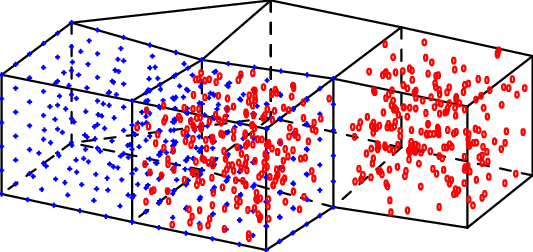
\includegraphics[width=0.7\textwidth]{./png/colpri.png}}
\caption{
\nep \ software will use finite elements and particles to represent different atomic species
as needed.
\label{fig:colpri}}
\end{figure}

In FM-WP2, a novel ``moment-based'' approach is being developed (for both
plasma species and neutrals).
This approach is a variant on gyrokinetics (though at present, the derivation
exists only for drift kinetics).
Instead of the stationary background Maxwellian of the usual gyrokinetics, this
approach uses a dynamically-varying background Maxwellian, where the
particle density, bulk velocity and temperatures are allowed to vary with time.
The result is a hybrid approach, where the software evolves both a fluid system
and a modified kinetic system.
One of the benefits of this approach is that it gives a natural means to
capture the fluid/kinetic transition, by switching between the fluid+kinetic
and fluid-only descriptions.
Moreover this approach allows the software to detect which of the fluid and kinetic
descriptions is valid in any region based on the properties of the modified
distribution function, and therefore to automatically evolve the relevant
model.

The favourable properties of this approach are valuable,
but as with any novel approach there is an inherent risk of the scheme not
working.  Thus as described in~\cite[\S\,1.1]{pappeqs2}, in the event that
this approach is not feasible, the kinetic calculations
will use a Particle-in-Cell (PIC) approach.
While full orbit PIC is potentially extremely expensive relative to gyrokinetics,
it has been very well-studied both in terms of theory and numerical implementation.
Moreover the issue of how to treat the transition from fluid to a particles in
a coupled model is well-understood, at least in classical fluid dynamics.

Relevant sheath physics boundary conditions are being derived as part of this
work, including shallow angles and collisions.
Ions which exit the domain re-enter as neutrals with the Knudsen cosine
distribution.

While the current derivation is electrostatic, there is nothing which precludes
the derivation of an electromagnetic model.


\subsubsection{Neutrals and impurities}

\paragraph{Different levels of multispecies capabilities should be considered.}
The framework nature of the code means this will be the case.

\paragraph{In medium to high fidelity models, neutrals and heavy species should
be treated fully kinetically (the former have potentially low collisionality
and they are not bound by the magnetic field, the latter have a large Larmor
radius).}

Development of a neutral gas and impurity model is ongoing under FM-WP3. 
Page 7 of the Science Plan states: {\green ``Kinetic levels of complexity are \ldots
necessary \ldots for modelling the burning plasma regime, due to the inherent
uncertainty in the fluid codes. 
The plasma in a fusion reactor may well behave significantly differently to
plasma in existing devices because it will in general contain two main ionic
species (Deuterium and Tritium), neutral fuel particles and ionised Helium ash
(or alpha particles), as well as impurity ions originating from the wall.''}
That is, kinetic models will be derived and implemented, though it is hoped
that this will facilitate the development of fluid models.

\paragraph{In high fidelity models, dynamical neutral evolution on the
turbulence time scale would be preferable, if possible.}
High-fidelity simulations will use a kinetic model for neutrals where appropriate. 

\paragraph{Ability to model pumps (either directly or via pumping surfaces)
should be included. Pellets: the code should enable simulation of, or coupling
to models that can model, pellet fuelling.}
Models for these aspects are not included in the Science Plan.
As we will use an unstructured mesh, it will be possible to describe arbitrary
pumping surfaces.

The role of sources and sinks is recognised to be crucial in \nep\ physics so
that modelling of pellets as a source will be possible.
The tool CWIPI (Coupling With Interpolation Parallel Interface) may be used for
coupling to more complicated pellet models.
